\subsection{GitHub ของหุ่นยนต์ฮิวมานอยด์ UTHAI}
ไฟล์ข้อมูลทุกอย่างเกี่ยวกับหุ่นยนต์ฮิวมานอยด์ UTHAIได้ถูกอัพโหลดขึ้นบนอินเทอร์เนต
โดยอัพโหลดไปไว้ที่ GitHub [https://github.com/UTHAI-Humanoid] และมีการเขียน Wiki การใช้งานเบื้องต้นเอาไว้
สำหรับนักศึกษาหรือนักวิจัยที่ต้องการพัฒนาต่อ 
\begin{figure}[!ht]
	\centering
	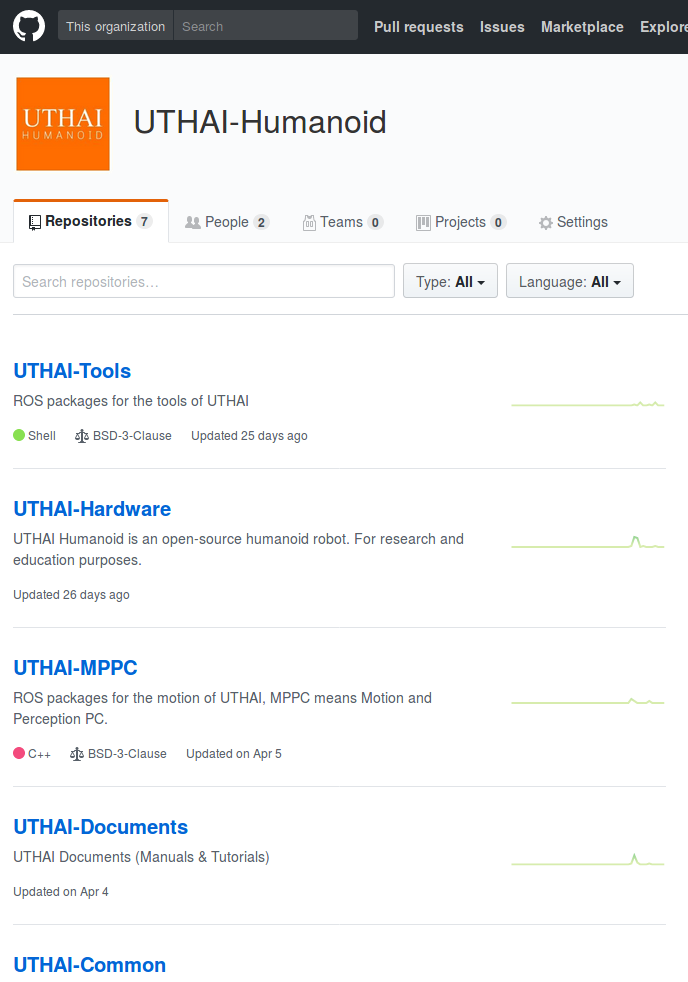
\includegraphics[width=0.42\textwidth]{chapter4/images/uthai_manual/uthai_github.png}
	\caption{GitHub ที่เก็บข้อมูลทั้งหมดของหุ่นยนต์ฮิวมานอยด์ UTHAI}
\end{figure}
\begin{figure}[!ht]
	\centering
	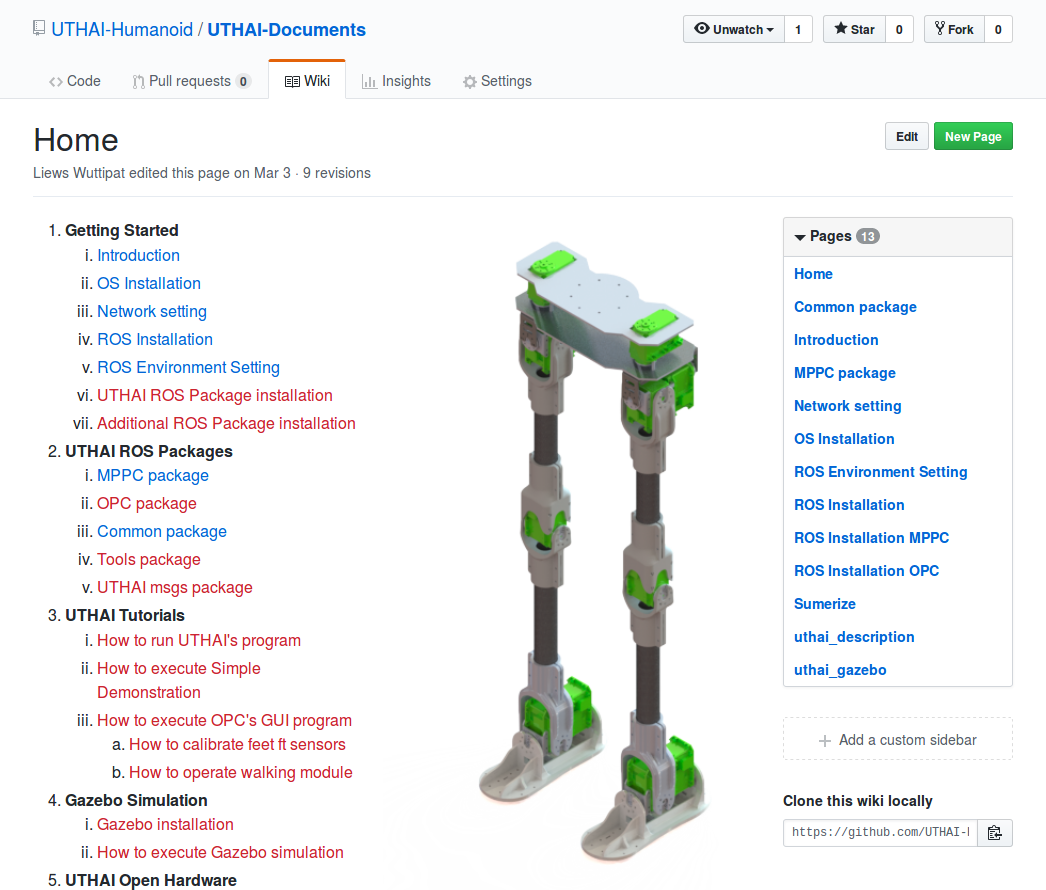
\includegraphics[width=0.60\textwidth]{chapter4/images/uthai_manual/uthai_github2.png}
	\caption{ตัวอย่าง Wiki การใช้งานเบื้องต้นของหุ่นยนต์ฮิวมานอยด์ UTHAI}
\end{figure}


\clearpage
\subsection{ตัวอย่างเฟรมของหุ่นยนต์ฮิวมานอยด์ UTHAI}
เฟรมของหุ่นยนต์ฮิวมานอยด์ UTHAIได้ถูกอัพโหลดให้อยู่บนอินเทอร์เน็ต โดยอยู่ที่ https://github.com/UTHAI-Humanoid/UTHAI-Hardware/tree/master/Mechanics/Frame

\begin{figure}[!ht]
	\centering
	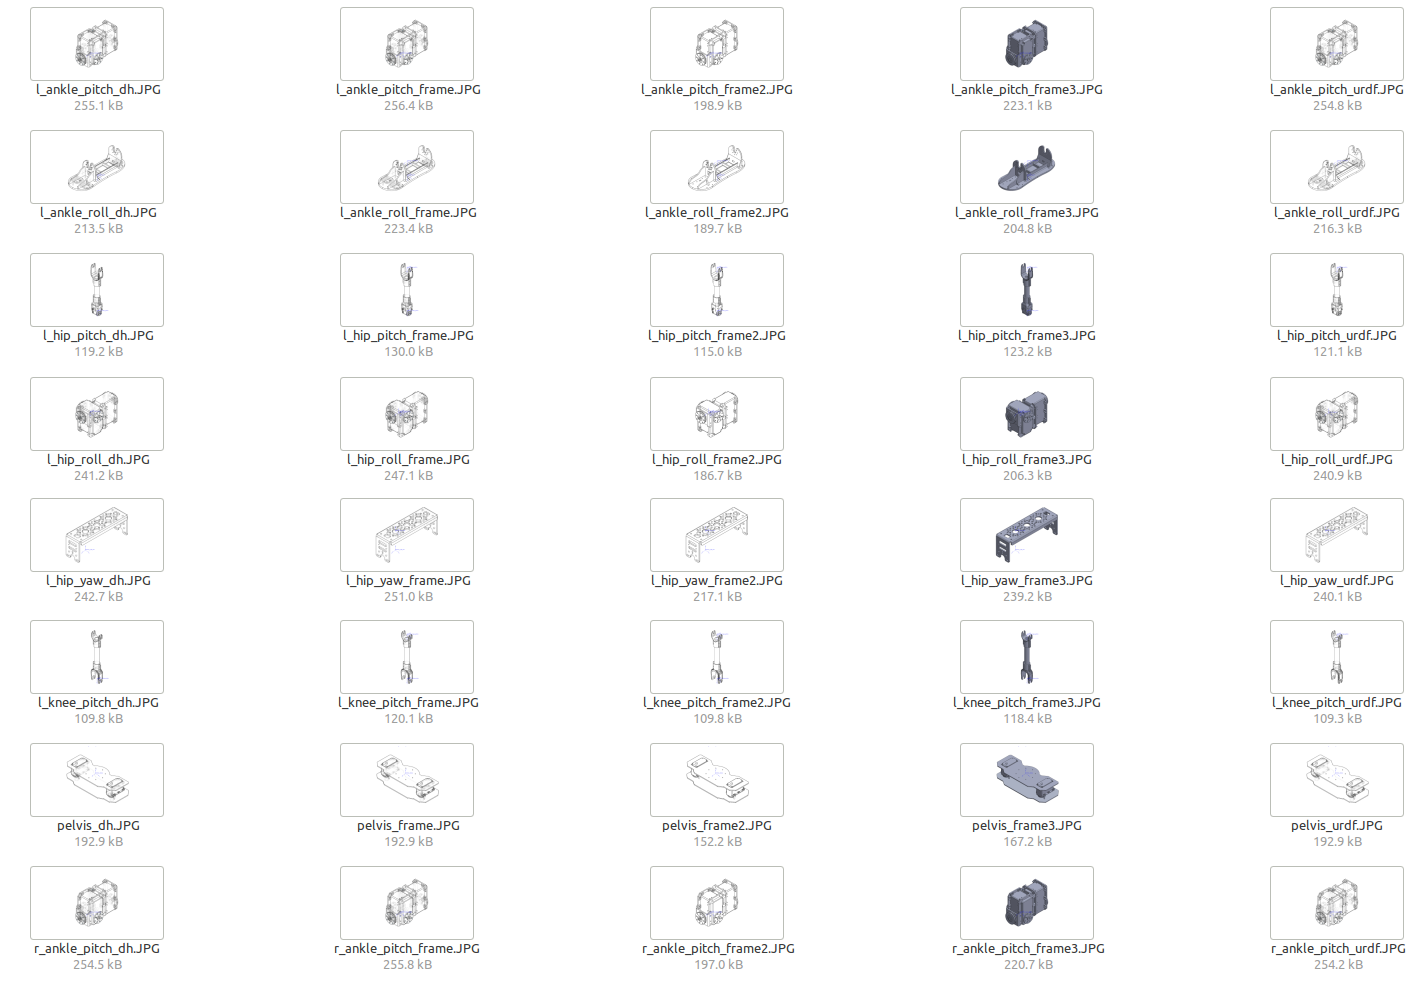
\includegraphics[width=0.85\textwidth]{chapter4/images/uthai_manual/uthai_frame.png}
	\caption{ภาพเฟรมของแต่ละพาร์ทของหุ่นยนต์ฮิวมานอยด์ UTHAI}
\end{figure}
\begin{figure}[!ht]
	\centering
	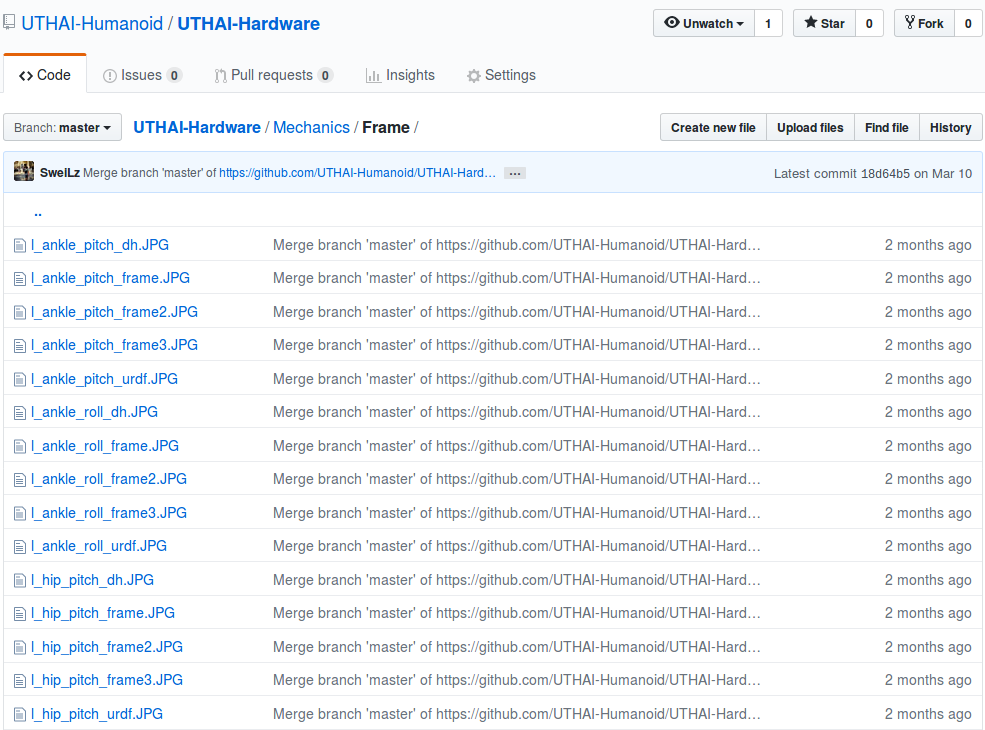
\includegraphics[width=0.85\textwidth]{chapter4/images/uthai_manual/uthai_frame2.png}
	\caption{ภาพ GitHub ของเฟรมแต่ละพาร์ทของหุ่นยนต์ฮิวมานอยด์ UTHAI}
\end{figure}

\clearpage
\subsection{ตัวอย่างเอกสารข้อมูลของหุ่นยนต์ฮิวมานอยด์ UTHAI}

\begin{figure}[!ht]
    \centering
    \begin{subfigure}[b]{0.45\textwidth}
        \centering
        
\includegraphics[width=\textwidth]{chapter4/images/uthai_manual/uthai_assembly.png}
        \caption{หน้าปกคู่มือการประกอบหุ่นยนต์ฮิวมานอยด์ UTHAI}
    \end{subfigure}
    \hfill
    \begin{subfigure}[b]{0.45\textwidth}
        \centering
        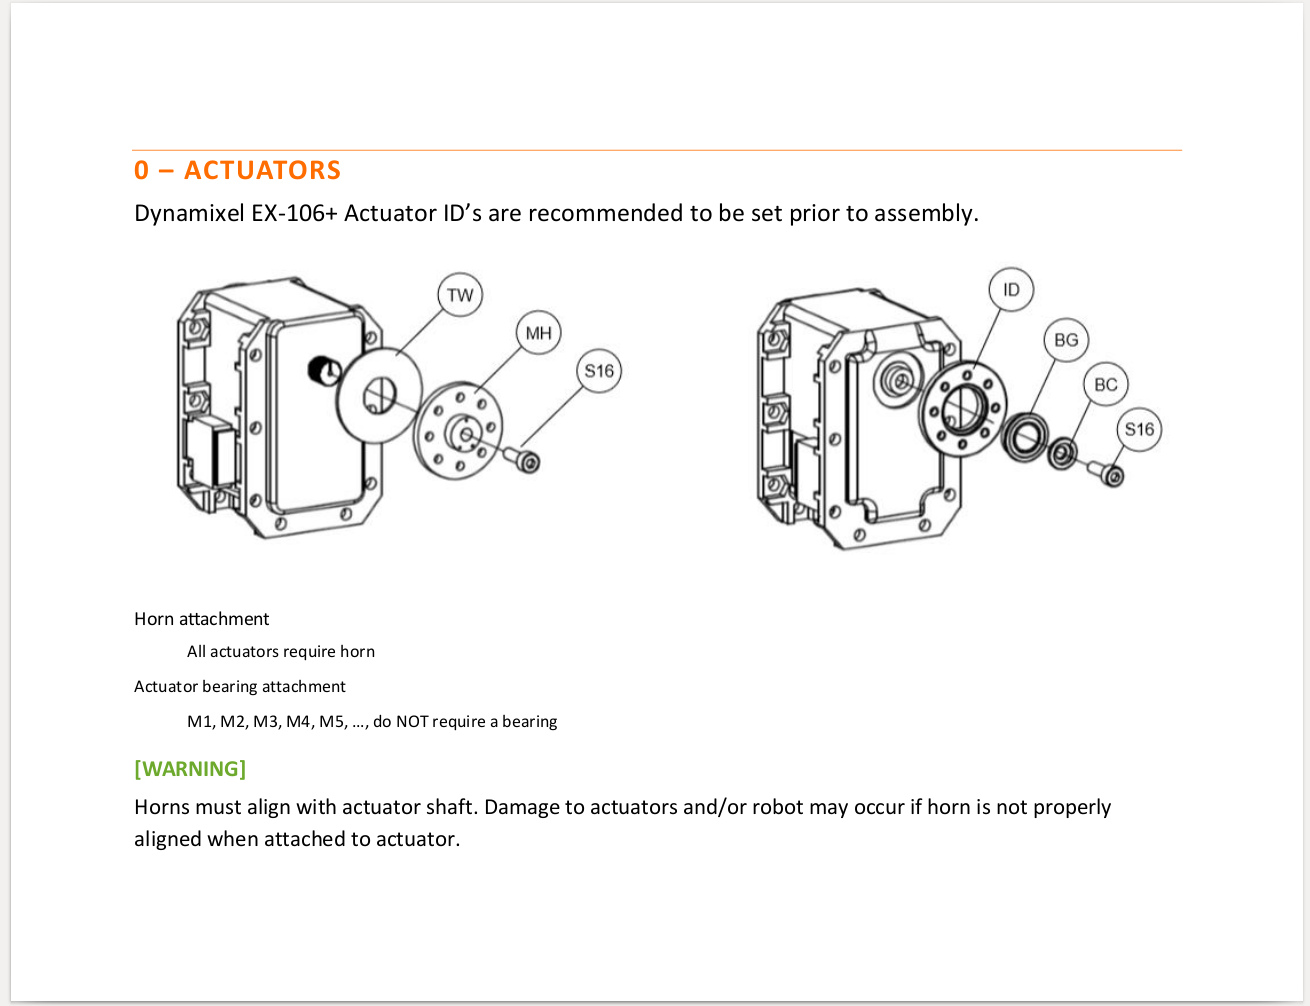
\includegraphics[width=\textwidth]{chapter4/images/uthai_manual/uthai_assembly2.png}
        \caption{ตัวอย่างคู่มือการประกอบหุ่นยนต์ฮิวมานอยด์ UTHAI}
    \end{subfigure}
    \caption{UTHAI Assembly Manual}
	\label{fig:uthai_assembly_manual}
\end{figure}
\begin{figure}[!ht]
    \centering
    \begin{subfigure}[b]{0.45\textwidth}
        \centering
        
\includegraphics[width=\textwidth]{chapter4/images/uthai_manual/uthai_kinematics.png}
        \caption{หน้าปกรายละเอียดของหุ่นยนต์ฮิวมานอยด์ UTHAI}
    \end{subfigure}
    \hfill
    \begin{subfigure}[b]{0.45\textwidth}
        \centering
        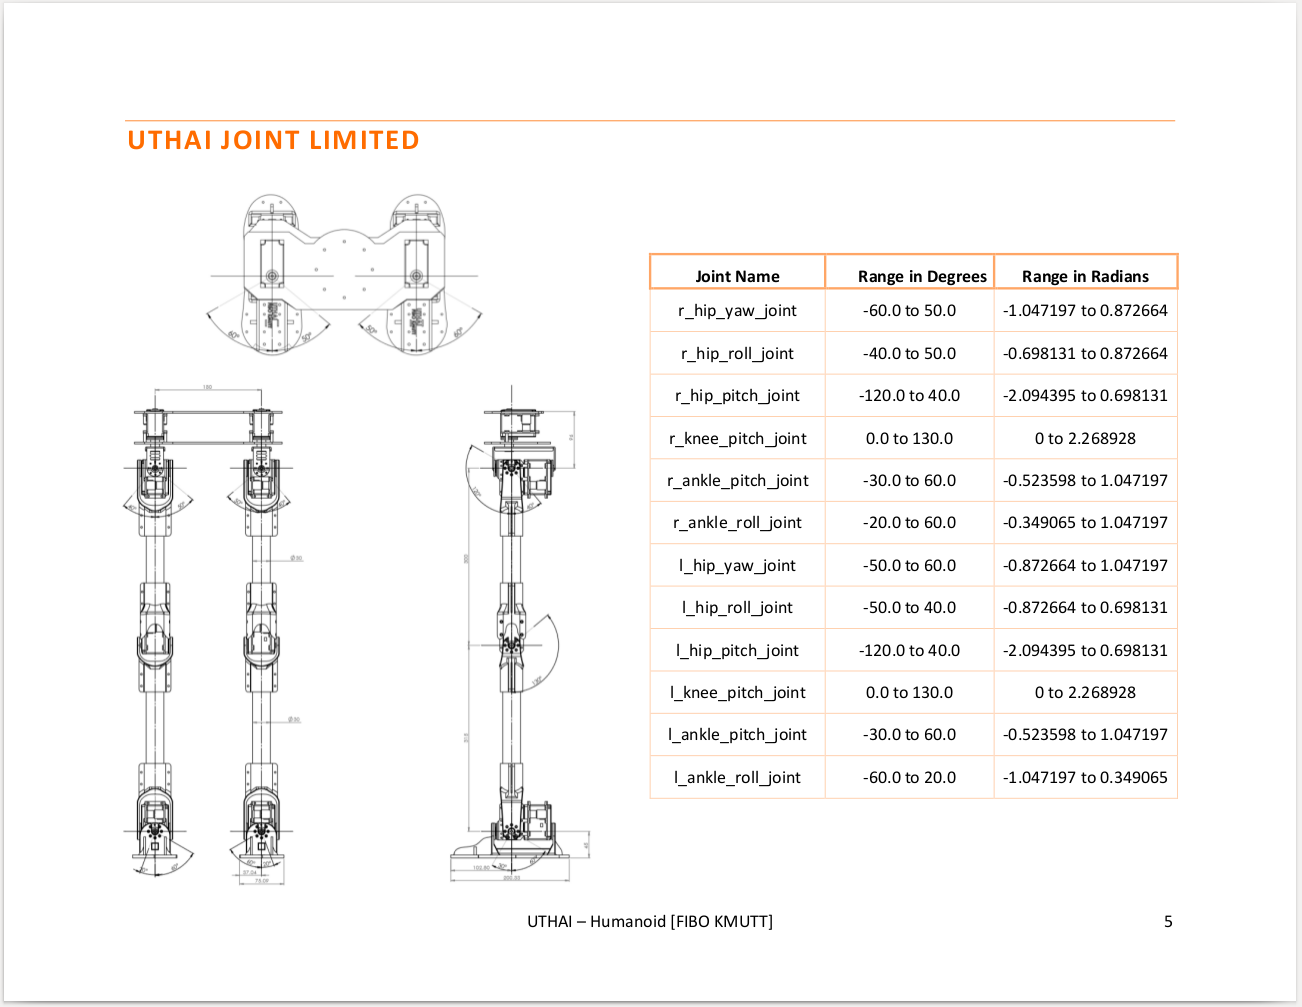
\includegraphics[width=\textwidth]{chapter4/images/uthai_manual/uthai_kinematics2.png}
        \caption{ตัวอย่างรายละเอียดของหุ่นยนต์ฮิวมานอยด์ UTHAI}
    \end{subfigure}
    \caption{UTHAI Kinematics Properties}
	\label{fig:uthai_kinematics_manual}
\end{figure}
\begin{figure}[!ht]
    \centering
    \begin{subfigure}[b]{0.45\textwidth}
        \centering
        
\includegraphics[width=\textwidth]{chapter4/images/uthai_manual/uthai_dynamics.png}
        \caption{หน้าปกรายละเอียดของหุ่นยนต์ฮิวมานอยด์ UTHAI}
    \end{subfigure}
    \hfill
    \begin{subfigure}[b]{0.45\textwidth}
        \centering
        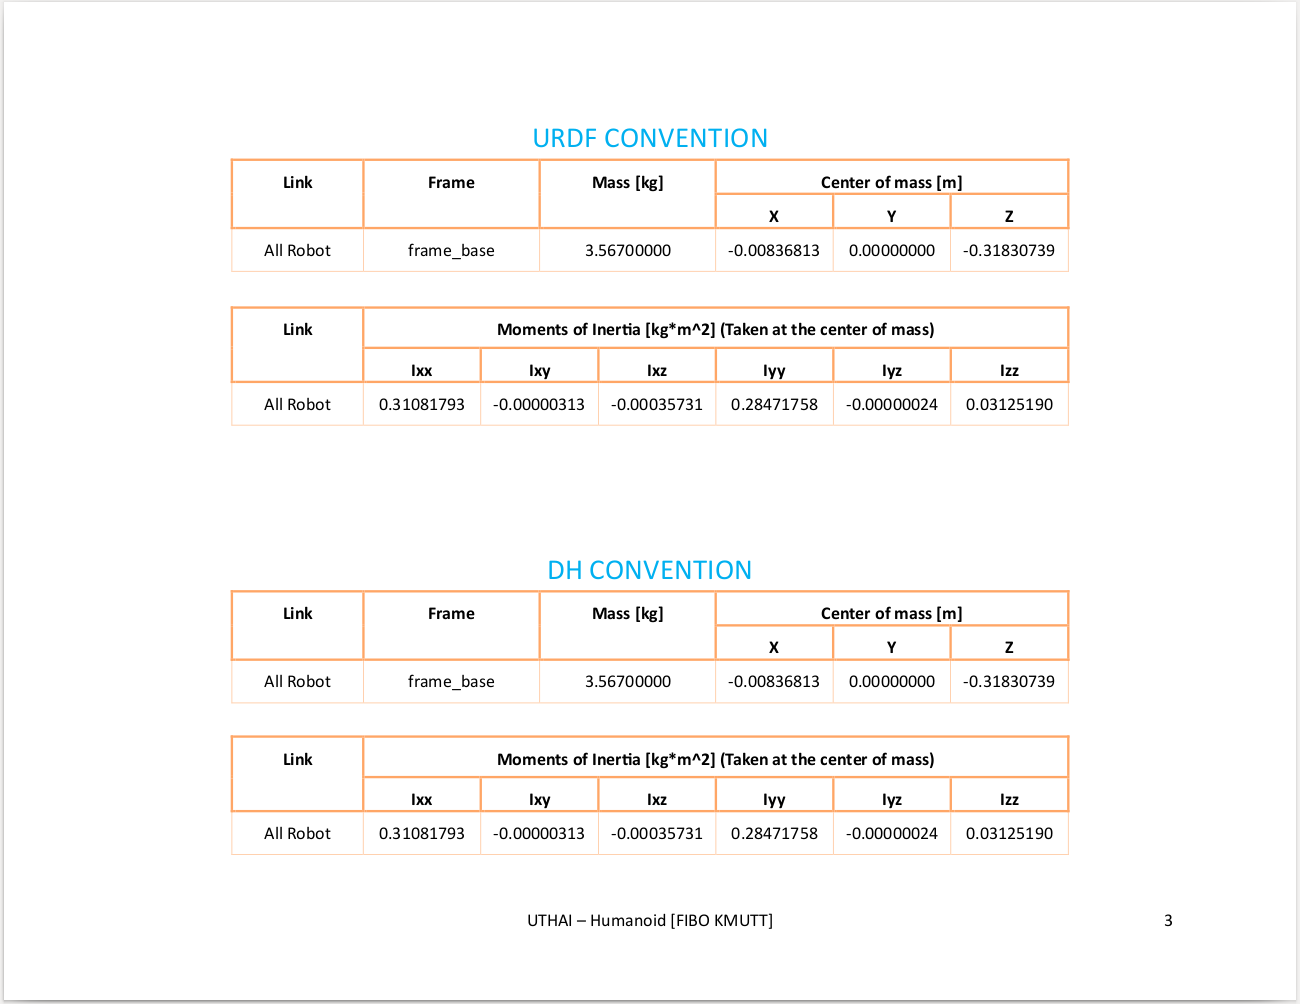
\includegraphics[width=\textwidth]{chapter4/images/uthai_manual/uthai_dynamics2.png}
        \caption{ตัวอย่างรายละเอียดของหุ่นยนต์ฮิวมานอยด์ UTHAI}
    \end{subfigure}
    \caption{UTHAI Dynamics Properties}
	\label{fig:uthai_dynamics_manual}
\end{figure}


\clearpage
\subsection{ภาพรวมระบบพื้นฐานของหุ่นยนต์ฮิวมานอยด์ UTHAI}
ระบบพื้นฐานที่ผู้วิจัยได้ทำการออกแบบก็เพื่อที่จะทำให้คนที่เข้ามาพัฒนาต่อยอดได้อย่างสะดวก และเป็นระบบระเบียบ
มีรูปแบบแบบแผน ซึ่งผู้วิจัยได้วางระบบนี้ขึ้นมาจากประสบการณ์การทำงานของผู้วิจัยเอง รวมถึงได้ค้นคว้าหาความรู้เพิ่มเติม
จนคิดว่าระบบนี้จะทำให้หุ่นยนต์ฮิวมานอยด์สามารถพัฒนาต่อได้ง่าย และเป็นประโยชน์ต่อผู้วิจัยท่านอื่นที่ต้องการนำระบบพื้นฐานนี้ไปใช้งาน

\begin{figure}[!ht]
	\centering
	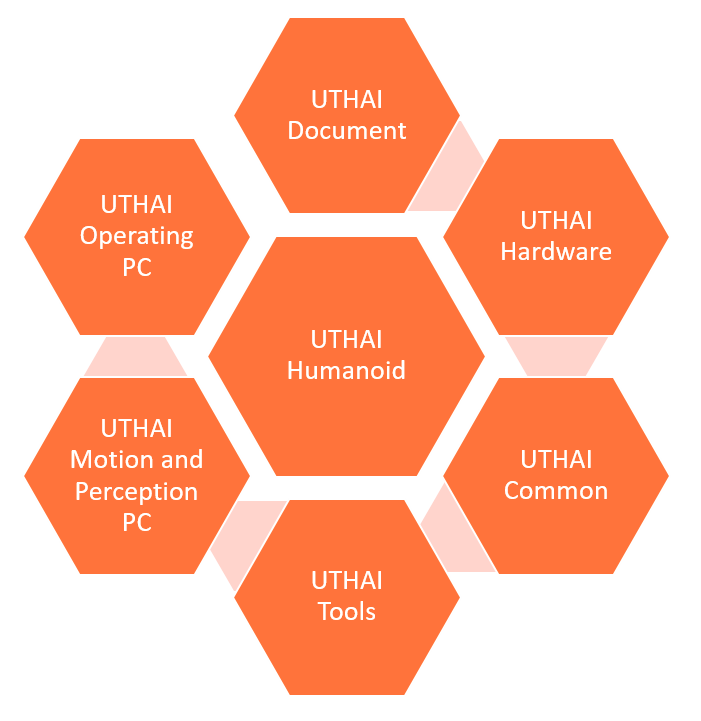
\includegraphics[width=0.7\textwidth]{chapter4/images/uthai_platform.png}
	\caption{ภาพรวมระบบพื้นฐานของหุ่นยนต์ฮิวมานอยด์ UTHAI}
	\label{fig:uthai_platform}
\end{figure}

ระบบพื้นฐานที่ผู้วิจัยออกแบบขึ้นมานั้น จะประกอบไปด้วยส่วนสำคัญอยู่ทั้งหมด 6 ส่วน คือ
\vspace{-10pt}
\begin{enumerate}[label=\arabic*., leftmargin=2.5cm]
    \setlength\itemsep{-0.25em}
    \item UTHAI-Documents
    \item UTHAI-Hardware
    \item UTHAI-Common
    \item UTHAI-MPPC
    \item UTHAI-OPC
    \item UTHAI-Tools
\end{enumerate}

\clearpage
\subsubsection*{UTHAI-Documents}
ในส่วนนี้คือส่วนของงานเอกสารต่างๆที่เกี่ยวข้องกับหุ่นยนต์ฮิวมานอยด์

\paragraph*{Reports-Hardware}
ใช้สำหรับเก็บรายงานวิทยานิพนธ์ทั้งฉบับร่างและฉบับสมบูรณ์ที่เกี่ยวข้องกับ การปรับเปลี่ยนโครงสร้างทางกล และทางไฟฟ้าของหุ่นยนต์ฮิวมานอยด์ UTHAI
\subparagraph*{- การออกแบบโครงสร้างและพัฒนาระบบพื้นฐานสำหรับหุ่นยนต์ฮิวมานอยด์เพื่อการศึกษาและวิจัย}

\paragraph*{Reports-Software}
ใช้สำหรับเก็บรายงานวิทยานิพนธ์ทั้งฉบับร่างและฉบับสมบูรณ์ที่เกี่ยวข้องกับการเพิ่มความสามารถของหุ่นยนต์ฮิวมานอยด์ UTHAI
\subparagraph*{- การพัฒนาระบบการเคลื่อนที่สำหรับหุ่นยนต์ฮิวมานอยด์}

\paragraph*{Wiki}
ใช้สำหรับเก็บ Tutorial ที่เกี่ยวกับการใช้งานของหุ่นยนต์ฮิวมานอยด์ UTHAI

\begin{figure}[!ht]
	\centering
	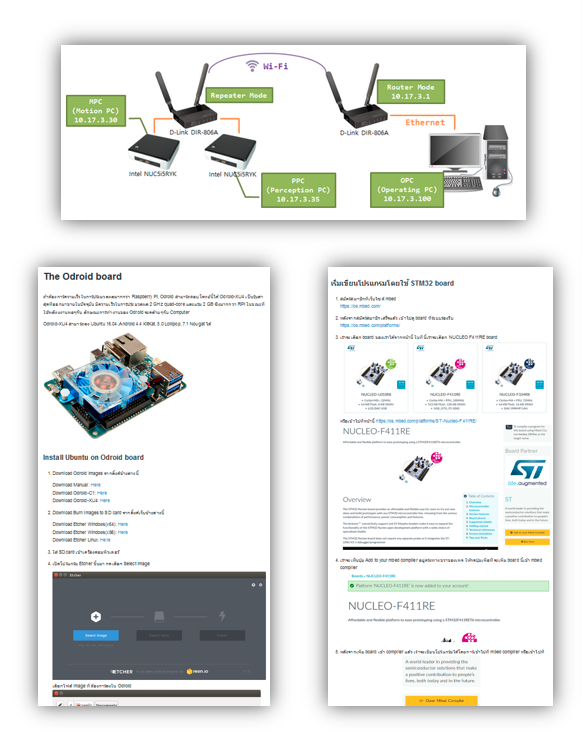
\includegraphics[width=0.7\textwidth]{chapter4/images/uthai_platform/uthai_doc.png}
	\caption{ภาพตัวอย่าง Tutorial ใน Wiki}
\end{figure}

ผู้วิจัยท่านอื่นสามารถที่จะช่วยกันเขียนและพัฒนาได้โดยการ Clone Repository แล้วทำการแก้ไขปรับปรุง หลังจากนั้นก็ Pull request ขึ้นมาเพื่อแสดงให้ผู้วิจัยท่านอื่นเห็นด้วย


\clearpage
\subsubsection*{UTHAI-Hardware}
ในส่วนนี้คือส่วนของรายละเอียดเกี่ยวกับโครงสร้างทั้งทางกลและทางไฟฟ้าที่เปิดให้ผู้วิจัยท่านอื่นสามารถนำไปประยุกต์ใช้ได้

\paragraph*{Drawing}
ไฟล์ออกแบบทางวิศวกรรมทุกชิ้นส่วนที่ต้องมีการขึ้นรูป
\paragraph*{STL files}
ไฟล์สำหรับการขึ้นรูปสามมิติและไฟล์สำหรับนำไปทำแบบจำลองหุ่นยนต์ฮิวมานอยด์
\paragraph*{Solidworks files}
ไฟล์ที่ออกแบบโดยใช้โปรแกรม Solidworks เพื่อให้นำไปแก้ไขปรับปรุงให้ดียิ่งขึ้นได้

\begin{figure}[!ht]
	\centering
	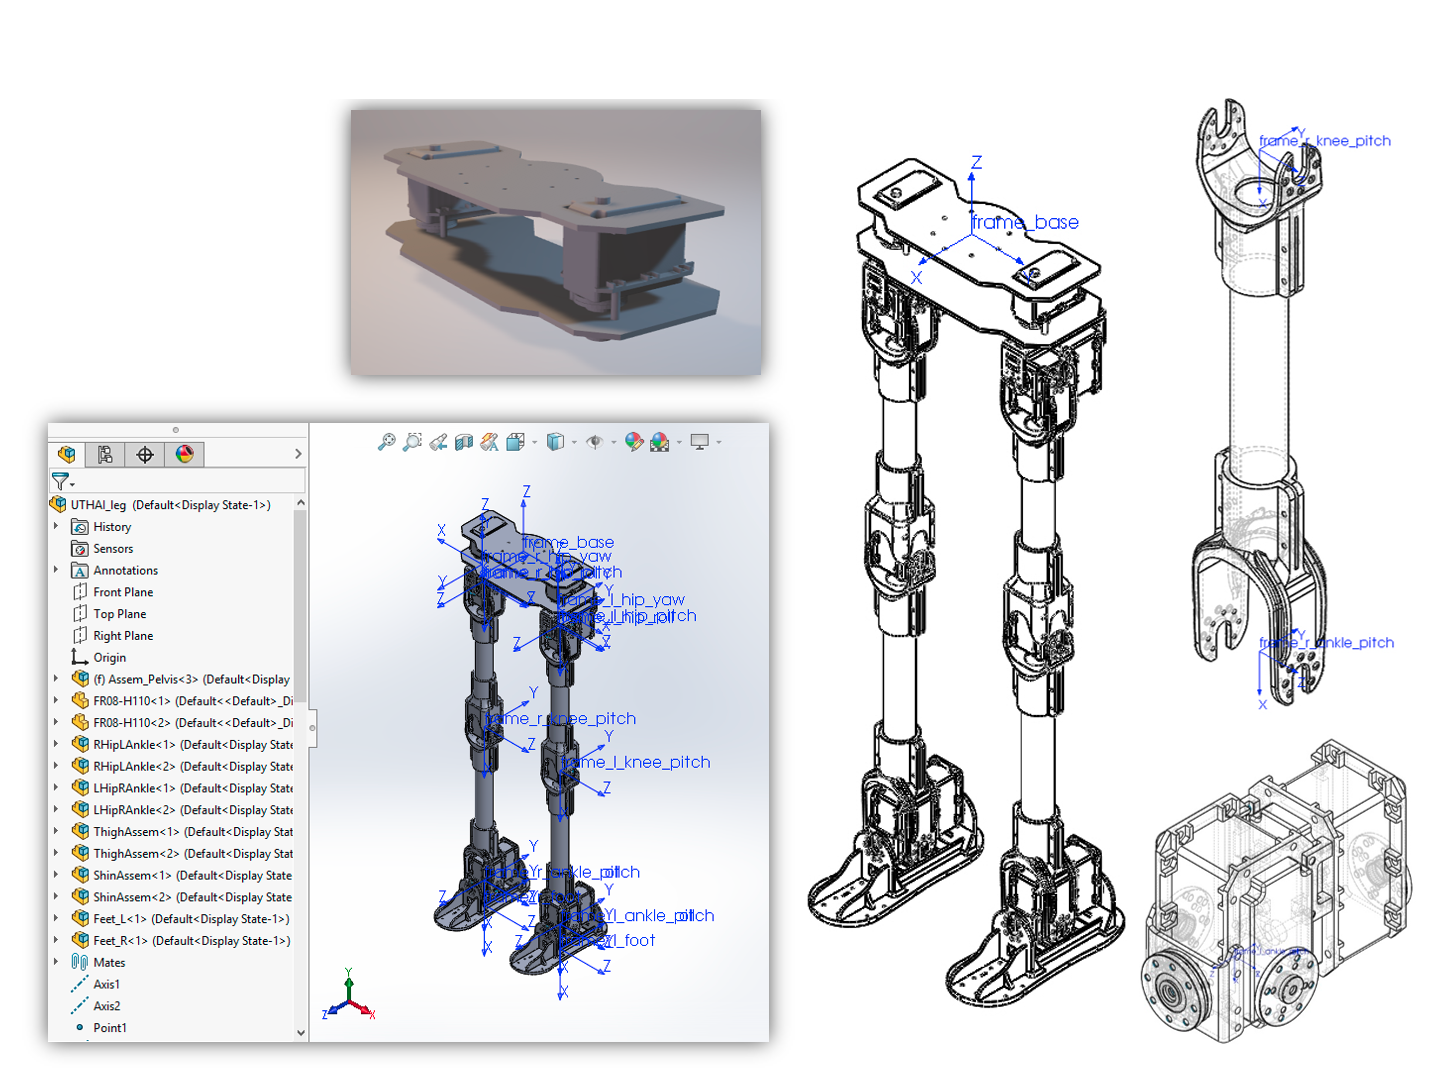
\includegraphics[width=0.8\textwidth]{chapter4/images/uthai_platform/uthai_hardware1.png}
	\caption{ภาพตัวอย่างไฟล์ใน UTHAI-Hardware}
\end{figure}
\begin{figure}[!ht]
	\centering
	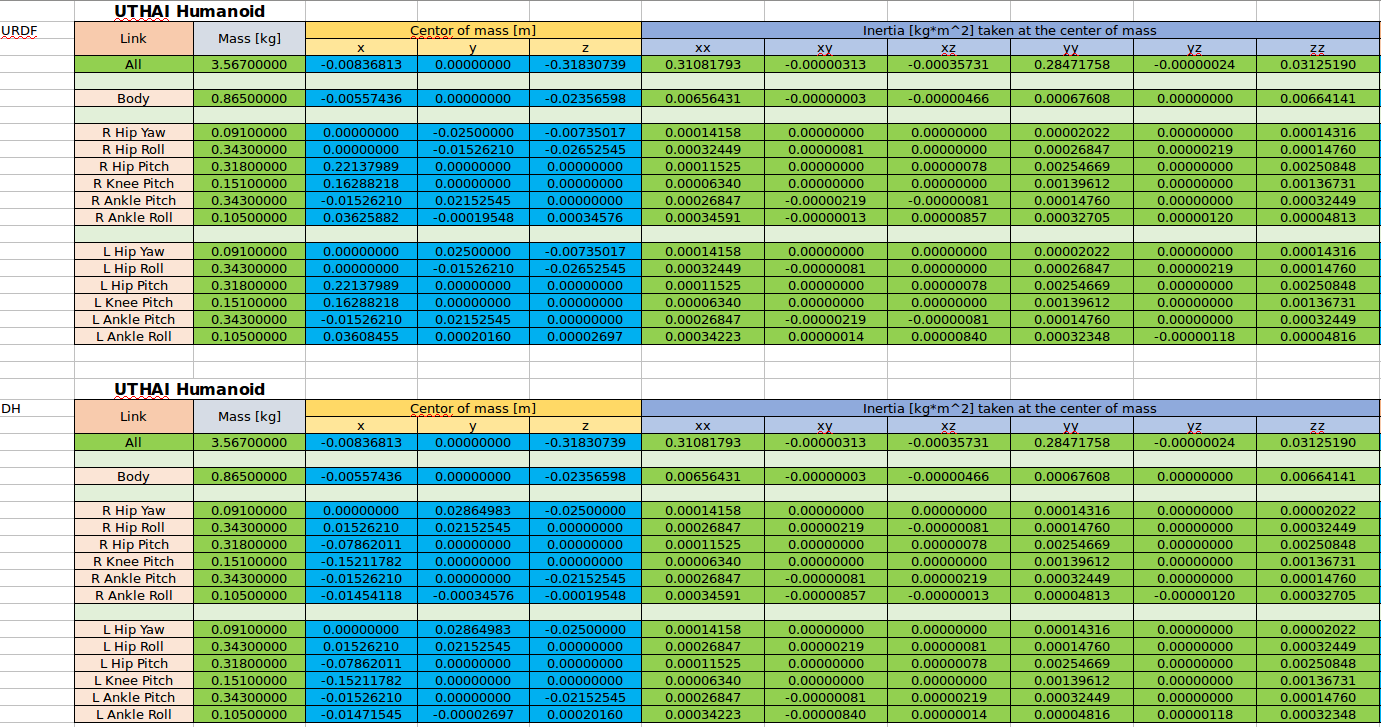
\includegraphics[width=0.8\textwidth]{chapter4/images/uthai_platform/uthai_properties.png}
	\caption{ภาพตัวอย่างไฟล์ใน UTHAI-Hardware}
\end{figure}


\clearpage
\subsubsection*{UTHAI-Common}
ในส่วนนี้คือส่วนของแพกเกจ ROS ที่ใช้เป็นพื้นฐานสำหรับการแสดงผลด้วยภาพ และระบบจำลองโดยจะมีแบบจำลองของหุ่นยนต์ฮิวมานอยด์ UTHAI ในรูปแบบของ URDF Xacro
\paragraph*{uthai\_description}
เป็นแพกเกจที่เขียนอธิบายลักษณะของหุ่นยนต์ฮิวมานอยด์เพื่อให้ ROS สามารถนำไปใช้ในกระบวนการอื่นได้
\paragraph*{uthai\_gazebo}
เป็นแพกเกจที่เอาไว้สำหรับทำระบบจำลองการทำงานของหุ่นยนต์ฮิวมานอยด์ UTHAI

\begin{figure}[!ht]
	\centering
	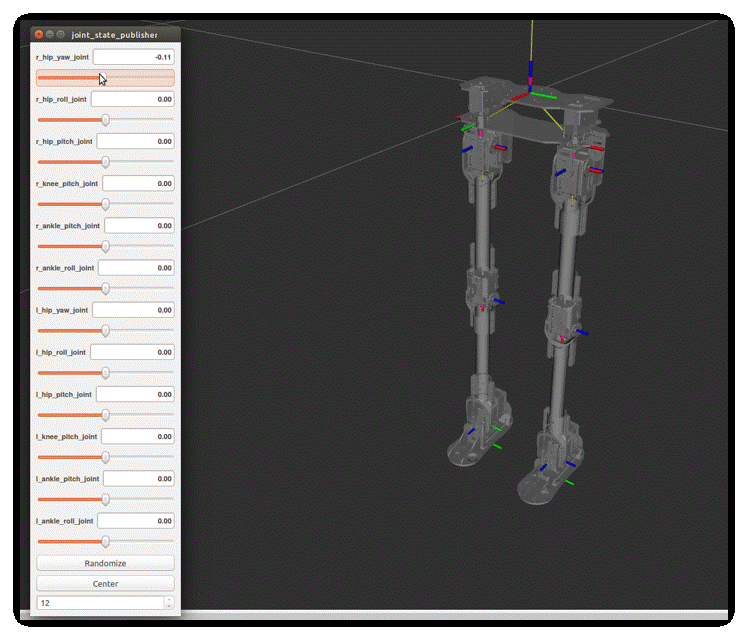
\includegraphics[width=0.6\textwidth]{chapter4/images/uthai_platform/uthai_rviz.png}
	\caption{ภาพ RViz ใน uthao\_description}
\end{figure}
\begin{figure}[!ht]
	\centering
	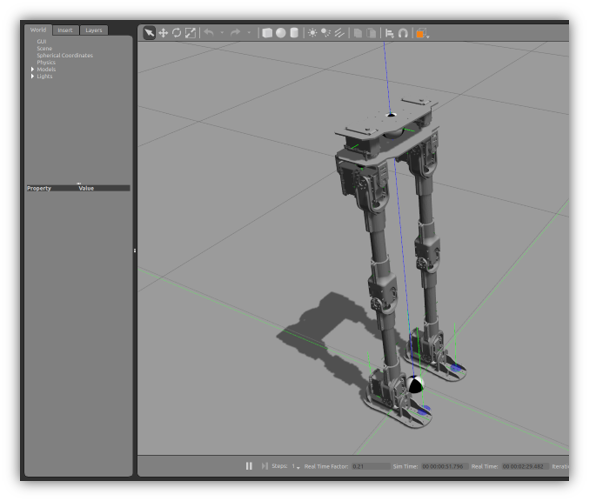
\includegraphics[width=0.6\textwidth]{chapter4/images/uthai_platform/uthai_gazebo.png}
	\caption{ภาพ Gazebo ใน uthai\_gazebo}
\end{figure}


\clearpage
\subsubsection*{UTHAI-MPPC}
ในส่วนนี้คือส่วนของแพกเกจ ROS ที่ใช้เป็นตัวในการเชื่อมต่อกับอุปกรณ์ฮาร์ดแวร์ของหุ่นยนต์ฮิวมานอยด์ UTHAI
เพื่อสั่งการตัวขับเคลื่อนดิจิตอลเซอร์โว และอ่านค่าเซนเซอร์จากตัวรับรู้หน่วยวัดความเฉื่อย การตรวจจับฝ่าเท้า
ตำแหน่งและความเร็วของตัวขับเคลื่อน
\paragraph*{uthai\_mbed}
เป็นแพกเกจที่เขียนเชื่อมต่อกับหน่วยประมวลผลระดับต่ำผ่าน rosserial เขียนด้วยภาษา python
โดยจะรับค่าเซนเซอร์หน่วยวัดความเฉื่อย เซนเซอร์ตรวจจับพื้น
\paragraph*{uthai\_manager}
เป็นแพกเกจที่เขียนเพื่อเอาไว้สำหรับจัดการตัวขับเคลื่อนทั้งหมด ให้สามารถสั่งการได้รวมถึง config ต่างๆด้วย
\paragraph*{uthai\_bringup}
เป็นแพกเกจที่เขียนเพื่อใช้ในการสั่งการตัวขับเคลื่อน ดิจิตอลเซอร์โว ที่เชื่อมต่อกับตัวประมวลผลระดับสูง

\begin{figure}[!ht]
	\centering
	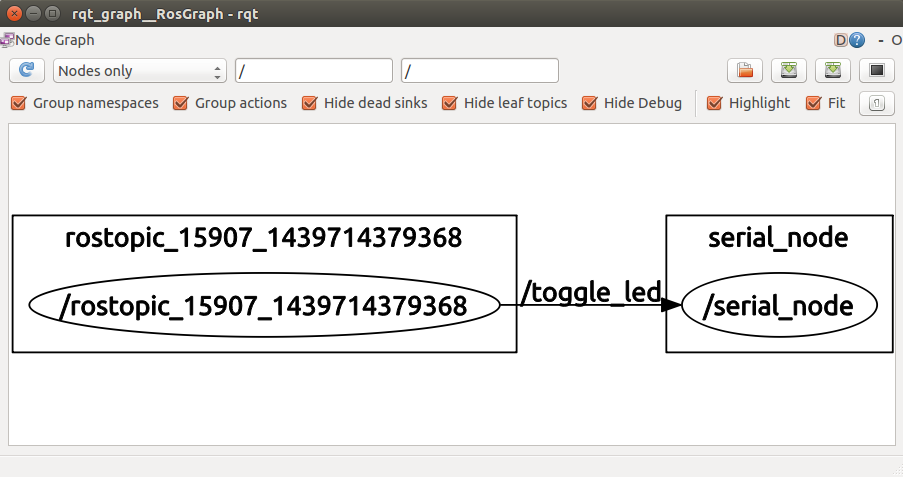
\includegraphics[width=0.8\textwidth]{chapter4/images/uthai_platform/ros_serial.png}
	\caption{ภาพ rqt\_graph ของ serial\_node}
\end{figure}


\subsubsection*{UTHAI-OPC}
ในส่วนนี้คือส่วนของแพกเกจ ROS ที่ใช้เป็นตัวในการเชื่อมต่อระหว่างตัวประมวลผลระดับสูงกับคอมพิวเตอร์ภายนอกเพื่อใช้ในการควบคุม
หรือการแสดงผลการทำงานที่ต้องใช้การคำนวณสูง เป็นการแบ่งเบาภาระการประมวลผลของตัวประมวลผลระดับสูง

\subsubsection*{UTHAI-Msgs}
ในส่วนนี้คือส่วนของแพกเกจ ROS ที่ใช้เป็นตัวในการเก็บ Messages ที่ใช้ในการติดต่อสื่อสารกันภายในระบบ ซึ่ง Messages ไม่เป็นมาตรฐาน
โดยอาจรวมไปถึง services และ actions ของระบบหุ่นยนต์ฮิวมานอยด์ UTHAIด้วย

\clearpage
\subsubsection*{UTHAI-Tools}
ในส่วนนี้คือส่วนของรายละเอียดเเครื่องมือที่ช่วยทำให้การทำงานมีประสิทธิภาพมากยิ่งขึ้น

\paragraph*{sketch-lib}
เป็นเครื่องมือที่ใช้สำหรับเอาไว้วาดรูปเฟรมของหุ่นยนต์
\begin{figure}[!ht]
    \centering
    \begin{subfigure}[b]{0.45\textwidth}
        \centering
        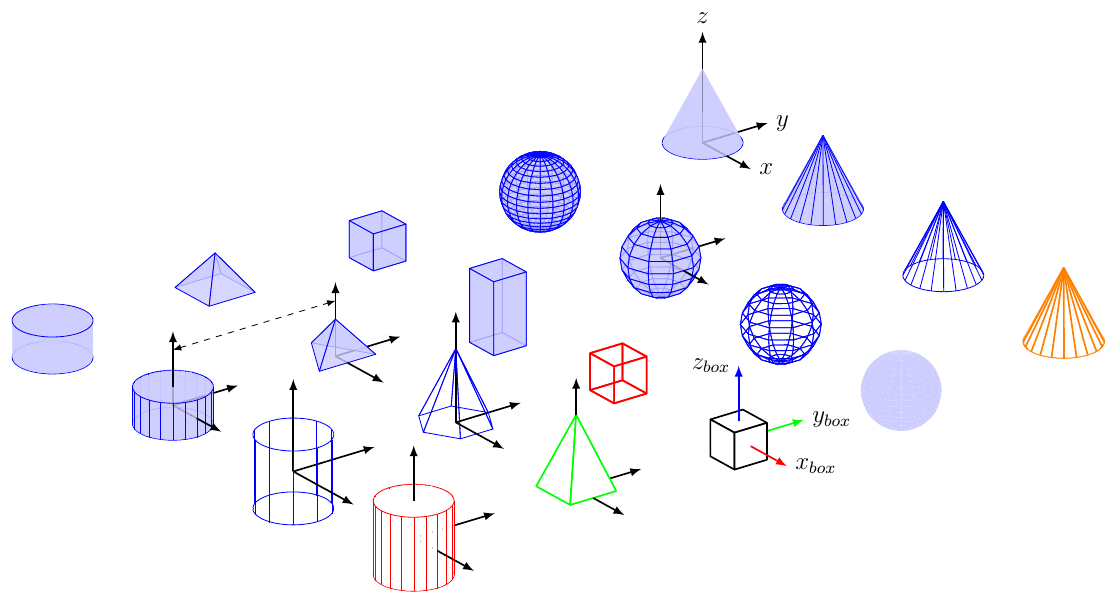
\includegraphics[width=\textwidth]{chapter4/images/uthai_tools/basic-shapes.png}
        \caption{ภาพตัวอย่างการวาดออฟเจ็คต่างๆ}
    \end{subfigure}
    \hfill
    \begin{subfigure}[b]{0.45\textwidth}
        \centering
        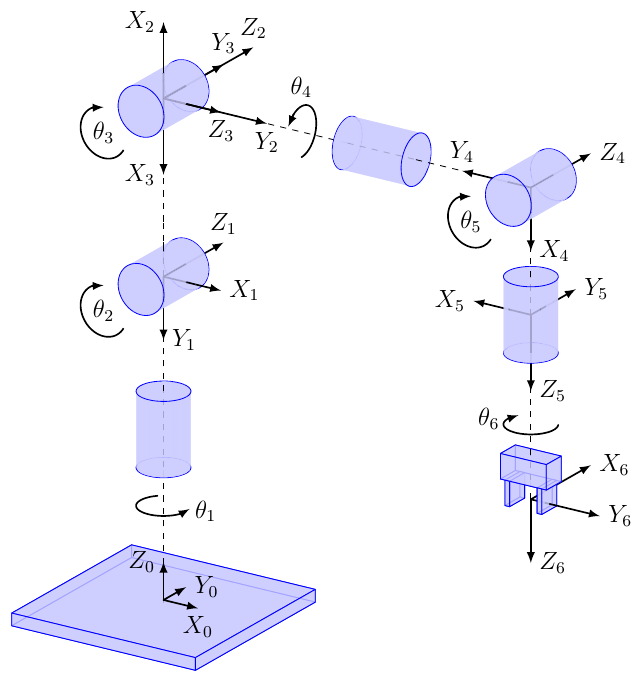
\includegraphics[width=\textwidth]{chapter4/images/uthai_tools/test_robot.png}
        \caption{ภาพตัวอย่างการวาดเฟรมของแขนกล}
    \end{subfigure}
    \caption{ภาพตัวอย่างการวาดเฟรมโดยใช้เครื่องมือนี้}
\end{figure}
\begin{figure}[!ht]
	\centering
	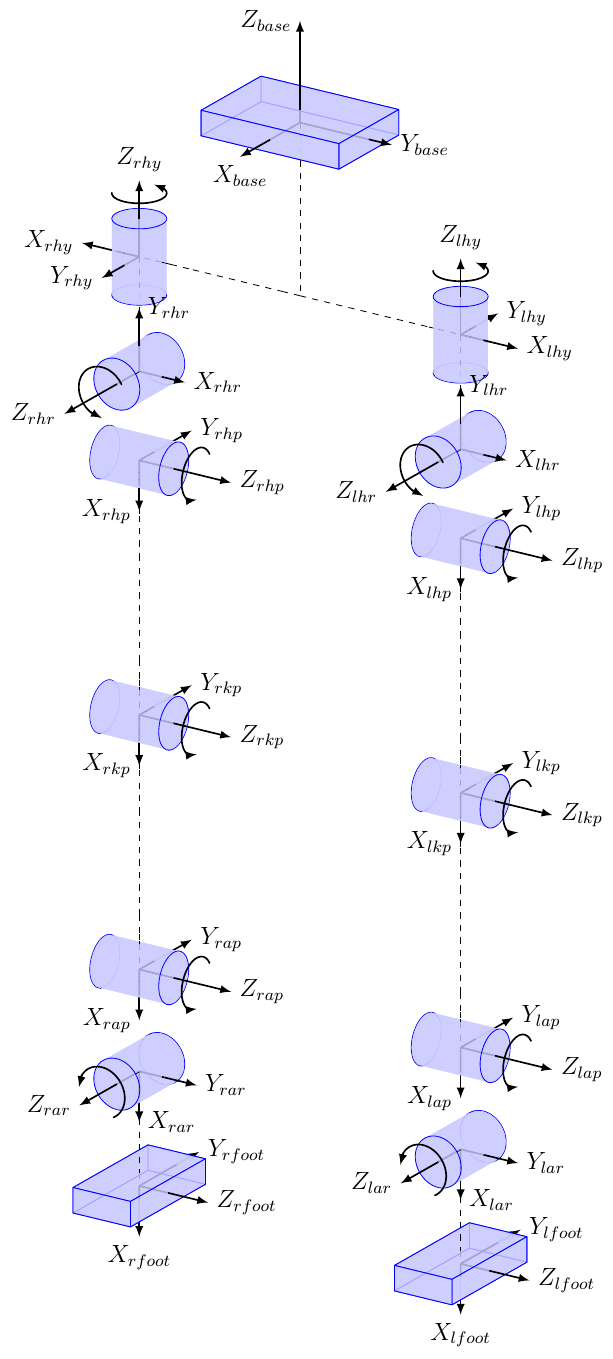
\includegraphics[width=0.3\textwidth]{chapter4/images/uthai_tools/uthai_kinematics.png}
	\caption{ภาพตัวอย่างการวาดเฟรมของหุ่นยนต์ฮิวมานอยด์}
	\label{fig:uthai_kinematics_sk}
\end{figure}